\documentclass[12pt]{ctexart}
\usepackage{amsmath}
\usepackage{listings}
\usepackage{subcaption}
\usepackage{graphicx}
\usepackage[dvipsnames]{xcolor}
\usepackage[backend=biber,style=gb7714-2015]{biblatex}

\lstset{
    basicstyle=\ttfamily\footnotesize,
    breaklines=true,
    keywordstyle=\bfseries\color{NavyBlue},
    commentstyle=\itshape\color{ForestGreen},
    stringstyle=\color{Apricot},
    columns=flexible,
    frame=single
}

\title{计算普朗特方程的数值解}
\author{***REMOVED*** \\ ***REMOVED***}

\addbibresource{references.bib}

\begin{document}
    \maketitle

\section{问题陈述}
我们知道,不可压缩的牛顿流体的流动满足纳维尔-斯托克斯方程:
\[
\left\{
\begin{aligned}
& \frac{\partial \vec U}{\partial t} + (\vec U \cdot \nabla) \vec U = - \frac{1}{\rho} \nabla p + \nu \nabla^2 \vec U + \vec f \\
& \nabla \cdot \vec U = 0
\end{aligned}
\right.
\]
该方程是一个复杂的非线性偏微分方程,其光滑解的存在性至今仍是未解之谜\cite{millenniumNSeq}。
为了更加方便地研究各种不同状态下流体的状态变化,流体力学家们一直在尝试简化该方程。

1909年,物理学家阿诺尔德·索末菲以奥斯鲍恩·雷诺的名字命名了一个新的常数,雷诺数,定义为\cite{sommerfeld1909beitrag}:
\[ \mathrm{Re} = \frac{Ul}{\nu} \]
雷诺数表征了流体的惯性作用和黏性作用之比\cite{10.1371/journal.pone.0141848},当其远大于1时,流体的惯性在流动中起主要作用,因此可以在一定程度上忽略黏性的作用,从而降低求解N-S方程的难度。

然而,N-S方程中的黏度项不仅与运动黏度$\nu$有关,还和流速的拉普拉斯算子有关,这意味着对速度梯度变化极快的区域,直接忽略黏性项会产生非常大的误差。
为了解决这一问题,流体力学家路德维希·普朗特提出了边界层的概念\cite{Tollmien1961}。
由于速度梯度的快速变化通常在壁面附近发生,他将高雷诺数的流体分为靠近壁面和远离壁面两个部分,并将靠近壁面的一部分称为边界层。
在边界层外,可以使用无黏性的近似来求解N-S方程;而在边界层内则依然需要考虑黏性。

普朗特利用量级分析将边界层中的N-S方程简化为以下方程:
\[
    \left\{
        \begin{aligned}
            & u \partial_x u + v \partial_y u = - \frac{1}{\rho} \partial_x p + \nu \partial_{yy} u \\
            & \partial_y p = 0 \\
            & \partial_x u + \partial_y v = 0
        \end{aligned}
    \right.
\]

我们考虑一侧为平板,另一侧为以固定速度流动的无黏性区域流体之间的边界层。
对无黏性的流体使用伯努利定律,可发现其压力不变,故$\partial_x p = 0$。
因此普朗特方程可进一步简化为:
\[
    \left\{
        \begin{aligned}
            & u \partial_x u + v \partial_y u = \nu \partial_{yy} u \\
            & \partial_x u + \partial_y v = 0
        \end{aligned}
    \right.
\]
我们将使用有限差分法求出该方程的数值解。

\section{有限差分法}

我们首先考虑动量方程,即第一个方程,因为该方程较为复杂。
注意到该方程是一个\emph{抛物偏微分方程},对$y$具有二阶偏导,而对$x$只具有一阶偏导,因此我们可以选择以$x$作为行进方向。
因此,我们将$u$沿$x$方向的导数写为后向差分,而将沿$y$方向的导数写成中间差分,该方程变为:
\[ 
    u_{x,y} \frac{u_{x+1, y} - u_{x,y}}{\Delta x} + v_{x,y} \frac{u_{x,y+1} - u_{x,y-1}}{2 \Delta y} = 
    \nu \frac{u_{x,y+1} - 2 u_{x, y} + u_{x,y-1}}{(\Delta y)^2}
\]
而质量连续性方程变为:
\[ \frac{u_{x+1,y} - u_{x,y}}{\Delta x} + \frac{v_{x+1,y} - v_{x+1,y-1}}{\Delta y} = 0 \]

因此,我们可以使用$u_{x,y+1}, u_{x, y}, u_{x,y-1}$来求解$u_{x+1,y}$。
注意到方程中还有一个未知数$v_{x,y}$,我们可以选择在计算$u$的同时利用连续性方程计算$v$,也可以选择先设$v$为某初始值,计算$u$,然后计算$v$,然后再迭代一次,重新计算。
第二种方法可称为预测-校正法,这种方法实现较为简单,因此我们选择这种方法。

为了求解边界层厚度,我们从靠近墙壁的方向向外迭代求解,并在流向速度大于一定阈值的时候中断。
流体力学中通常以自由流速的$99\%$作为阈值,此处我们取$99.95\%$。

\subsection{全显式法}

将第一个方程移项,可得:
\[ 
    u_{x+1,y} = \frac{\Delta x}{u_{x,y}} 
    \left( 
        \nu \frac{u_{x,y+1} - 2 u_{x, y} + u_{x,y-1}}{(\Delta y)^2}  
        - v_{x,y} \frac{u_{x,y+1} - u_{x, y-1}}{2 \Delta y} + \frac{u_{x,y} u_{x,y}}{\Delta x}
    \right) 
\]
正如上文所述,若需要求解$u_{x+1,y}$,我们需要先求出$u_{x,y+1}, u_{x, y}, u_{x,y-1}$,这意味着我们只能先沿$x$轴前进,再沿$y$轴前进。
只有这样才能保证在计算$u_{x+1, y}$时需要的值都已经求出。

同理,$v_{x+1,y}$也可以使用这种方法求解。

这种方式即为全显式法,其易于实现,不需要求解复杂的线性或非线性方程组,因此通常不需要进行迭代。

然而,其缺点在于稳定性不足。该方法的稳定性约束为\cite{book:9105}:
\[ \frac{2\nu \Delta x}{u_{x,y} (\Delta y)^2} \le 1 \quad \text{且} \quad \frac{v_{x,y}^2 \Delta x}{u_{x,y} \nu} \le 2 \]
可以注意到若网格在$y$方向上划分过细,则该算法反而会不稳定。
此外,该方法的稳定性也与求出的解有关,这意味着我们必须调整参数才能获得稳定的解。
这些问题促使我们寻找更优秀的算法。

\subsection{Du Fort-Frankel法}

为了解决全显式法的不稳定的问题,同时保持显式方法易于理解、编写和求解的优点,Du Fort和Frankel提出了一个更稳定的解决方案\cite{du1953stability}。
对于欲在$x$方向上使用步进方法求解的物理量$\phi_{x+1,y}$,可使用其在$x$方向上的平均来替代$\phi_{x, y}$,即在方程中将所有$\phi_{x,y}$代替为:
\[ \overline{\phi_{x,y}} = \frac{\phi_{x+1,y} + \phi_{x-1,y}}{2} \]

现在可以重写动量方程:
\begin{multline*}
    \frac{u_{x+1,y} + u_{x-1,y}}{2 \Delta x} \left( u_{x+1,y} - \frac{u_{x+1,y}+u_{x-1,y}}{2} \right) \\
    + v_{x,y} \frac{u_{x, y+1} - u_{x, y-1}}{2 \Delta y} \\
    = \frac{\nu}{(\Delta y)^2} (u_{x,y+1} - u_{x+1,y} - u_{x-1,y} + u_{x,y-1})
\end{multline*}
这是一个关于$u_{x+1, y}$的二次方程,其写成标准形式$ax^2+bx+c=0$后的系数为:
\[
    \begin{aligned}
        a &= \frac{1}{4 \Delta x} \\
        b &= - \frac{\nu}{(\Delta y)^2} \\
        c &= - \frac{u_{x-1,j}^2}{4 \Delta x} - \frac{\nu}{\Delta y^2} \left( u_{x,y+1} + u_{x,y-1} - u_{x-1,y} \right) + v_{x,y} \frac{u_{x, y+1} - u_{x, y-1}}{2 \Delta y}
    \end{aligned}
\]
注意到$v_{x,y}$极小,因此可认为$c$是负数,总和$a$异号,因此该二次方程的判别式应当总是大于零。
实践表明在$y$轴网格不太细的情况下,该方程总是能求出实数解。
注意到在$a,c$异号时,根据韦达定理,二次方程的两个解的必然\emph{异号},我们总是选择正的那个解。

这种方法对稳定性的要求进一步降低。

\subsection{精确解}

我们对边界层方程的简化最早由普朗特的学生布拉休斯提出,这种简化允许我们求出边界层厚度的精确解\cite{blasius1907grenzschichten}。
通过寻找方程的相似性、进行无量纲化并引入流函数,可将普朗特方程转化成一个三阶非线性全微分方程,这种方程可以比较容易地使用数值方法(如打靶法)求解。

除去用数值方法求解速度之外,还可以直接代入定义求出边界层厚度。
以该方法求出的边界层厚度(自由流速$u_\infty$的$99\%$)为:
\[ \delta = 5.0 \sqrt{\frac{\nu x}{u_\infty}} \]

我们可以使用该结论来验证求解的正确性。

\section{结论}

\subsection{准确性}
取流向长度为$x = 10$,划分$1000$个网格,法向高度为$y = 0.005$,划分$50$个网格。
设动力粘度为$\nu = 10^{-6}$,自由流速为$u_\infty = 10$,然后进行求解,可得以下结果。

\begin{figure}[ht]
    \centering
    \begin{subfigure}{0.4\textwidth}
        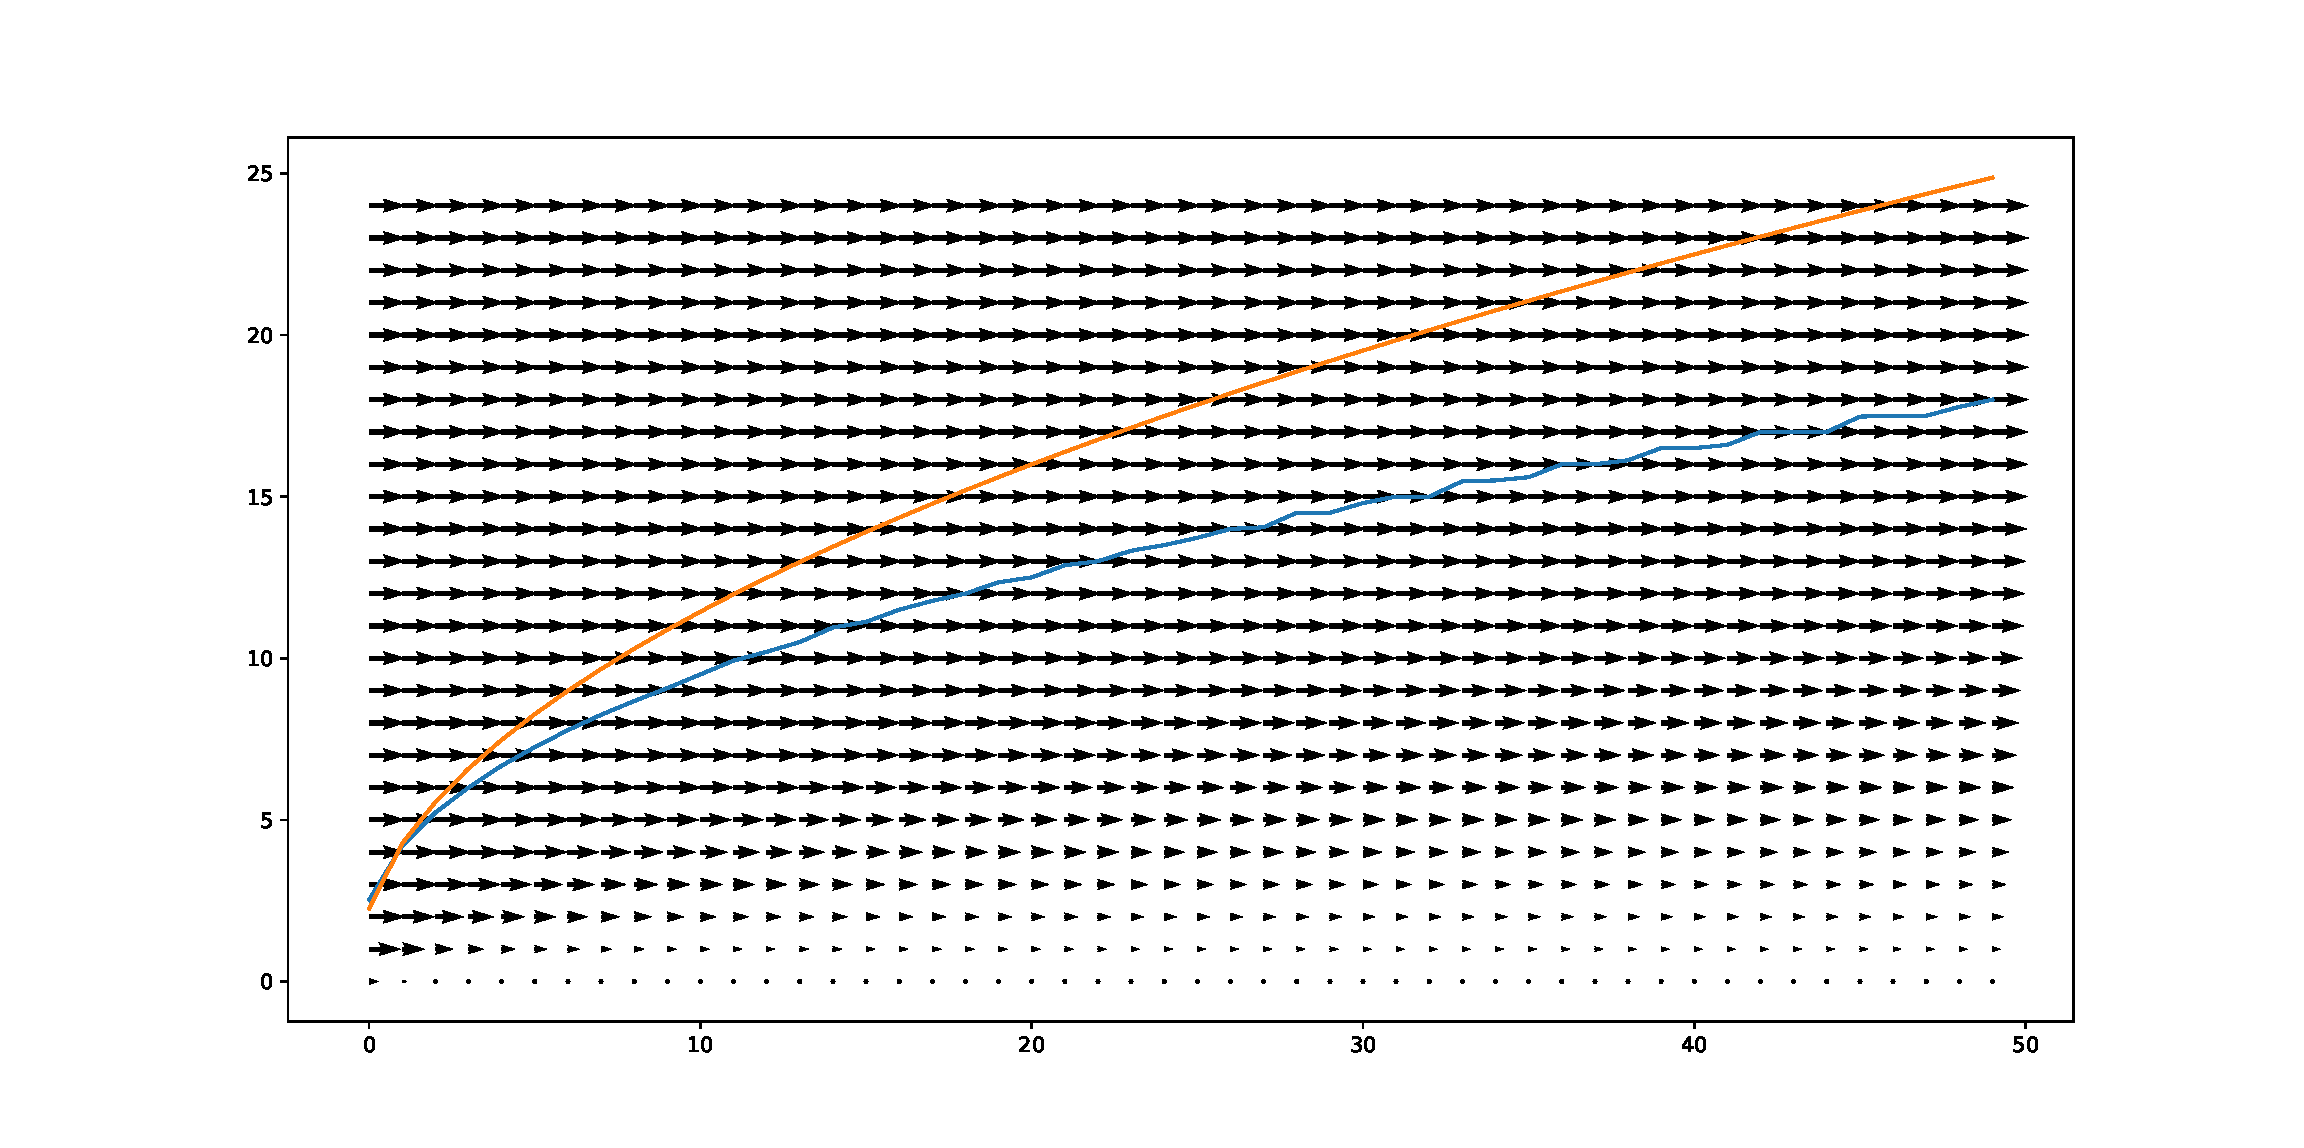
\includegraphics[width=\textwidth]{figure/explicit_with_exact_solution}
        \subcaption{全显式法}
    \end{subfigure}
    \begin{subfigure}{0.4\textwidth}
        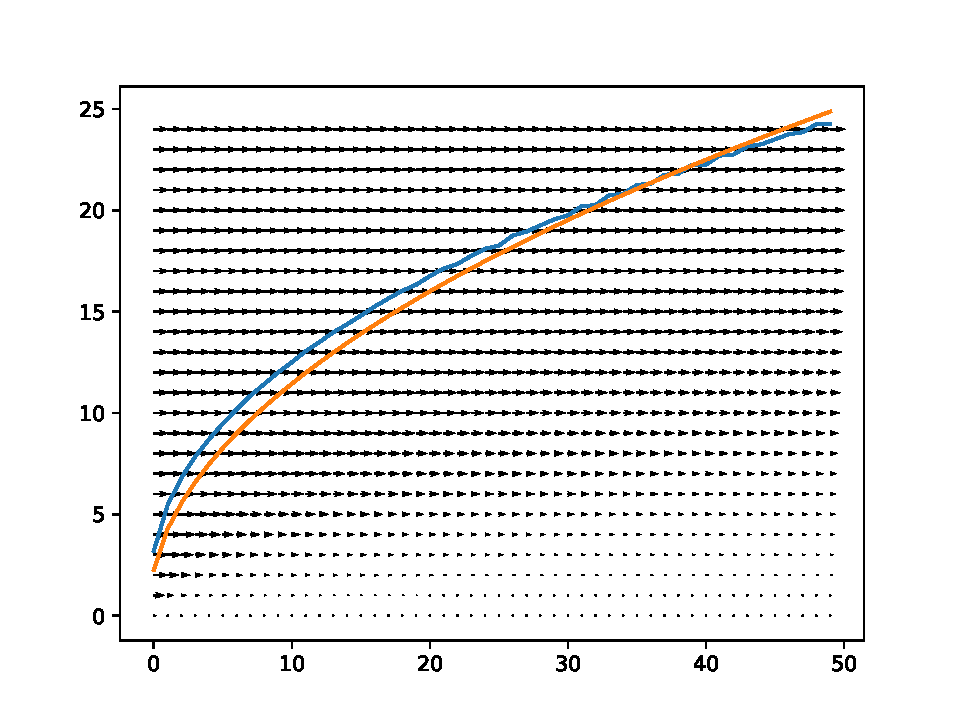
\includegraphics[width=\textwidth]{figure/dufort_with_exact_solution_2_iters}
        \subcaption{DuFort-Frankel法}
    \end{subfigure}
    \caption{数值解的速度场和边界层厚度,橙色线为精确解}
\end{figure}

可以发现,DuFort-Frankel法比全显式法的误差更小,更加接近精确解。

\subsection{稳定性}

我们已经知道,当$y$方向网格过密或速度过大时,全显式法不能得到稳定的解,我们构造了一组特别的数据以说明该问题。
\begin{figure}[ht]
    \centering
    \begin{subfigure}{0.4\textwidth}
        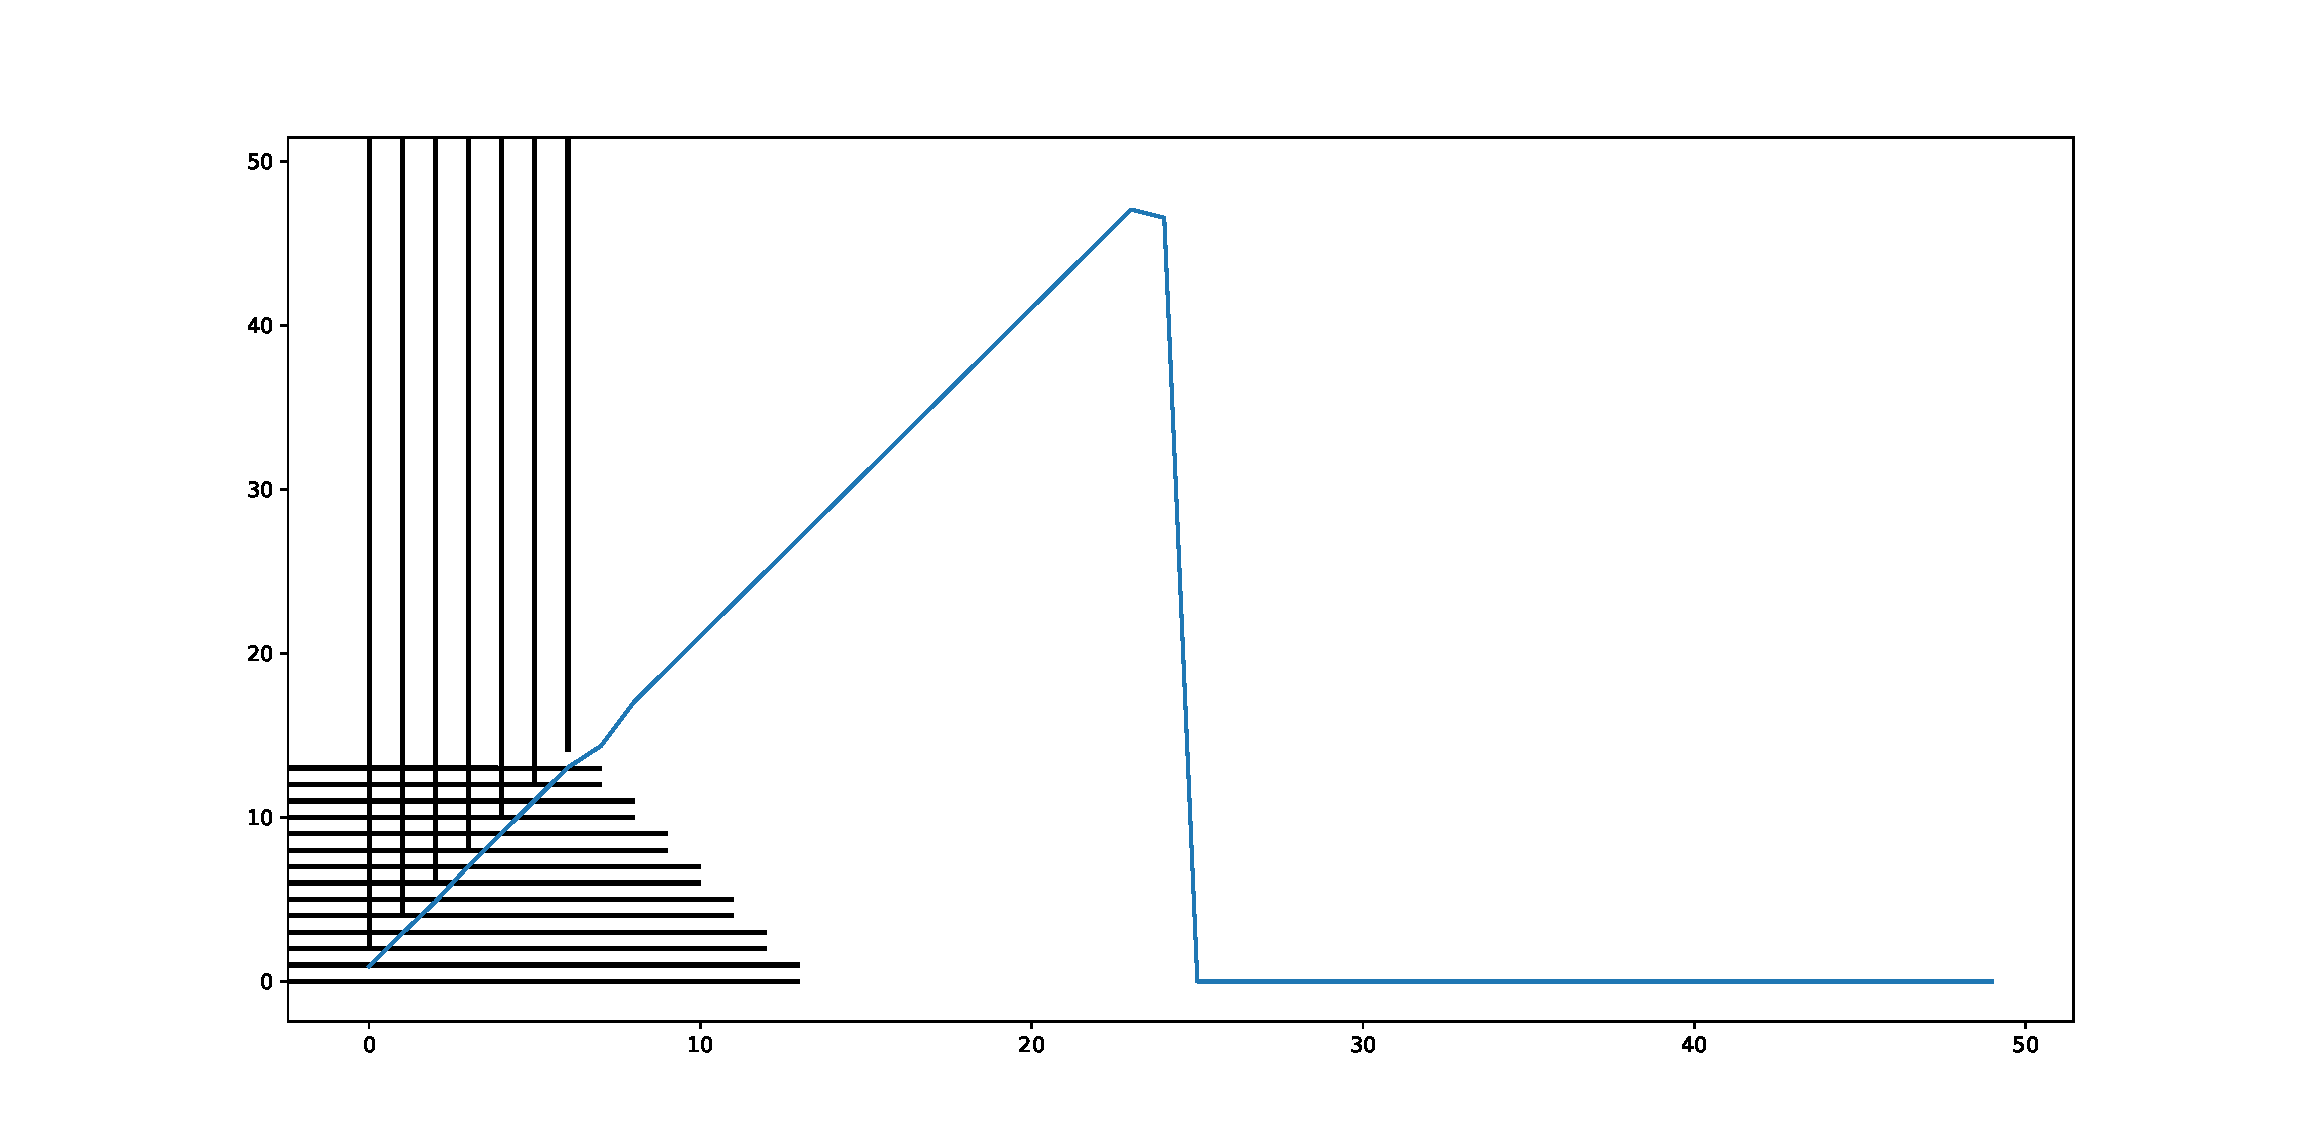
\includegraphics[width=\textwidth]{figure/explict_unstable.pdf}
        \subcaption{全显式法}
    \end{subfigure}
    \begin{subfigure}{0.4\textwidth}
        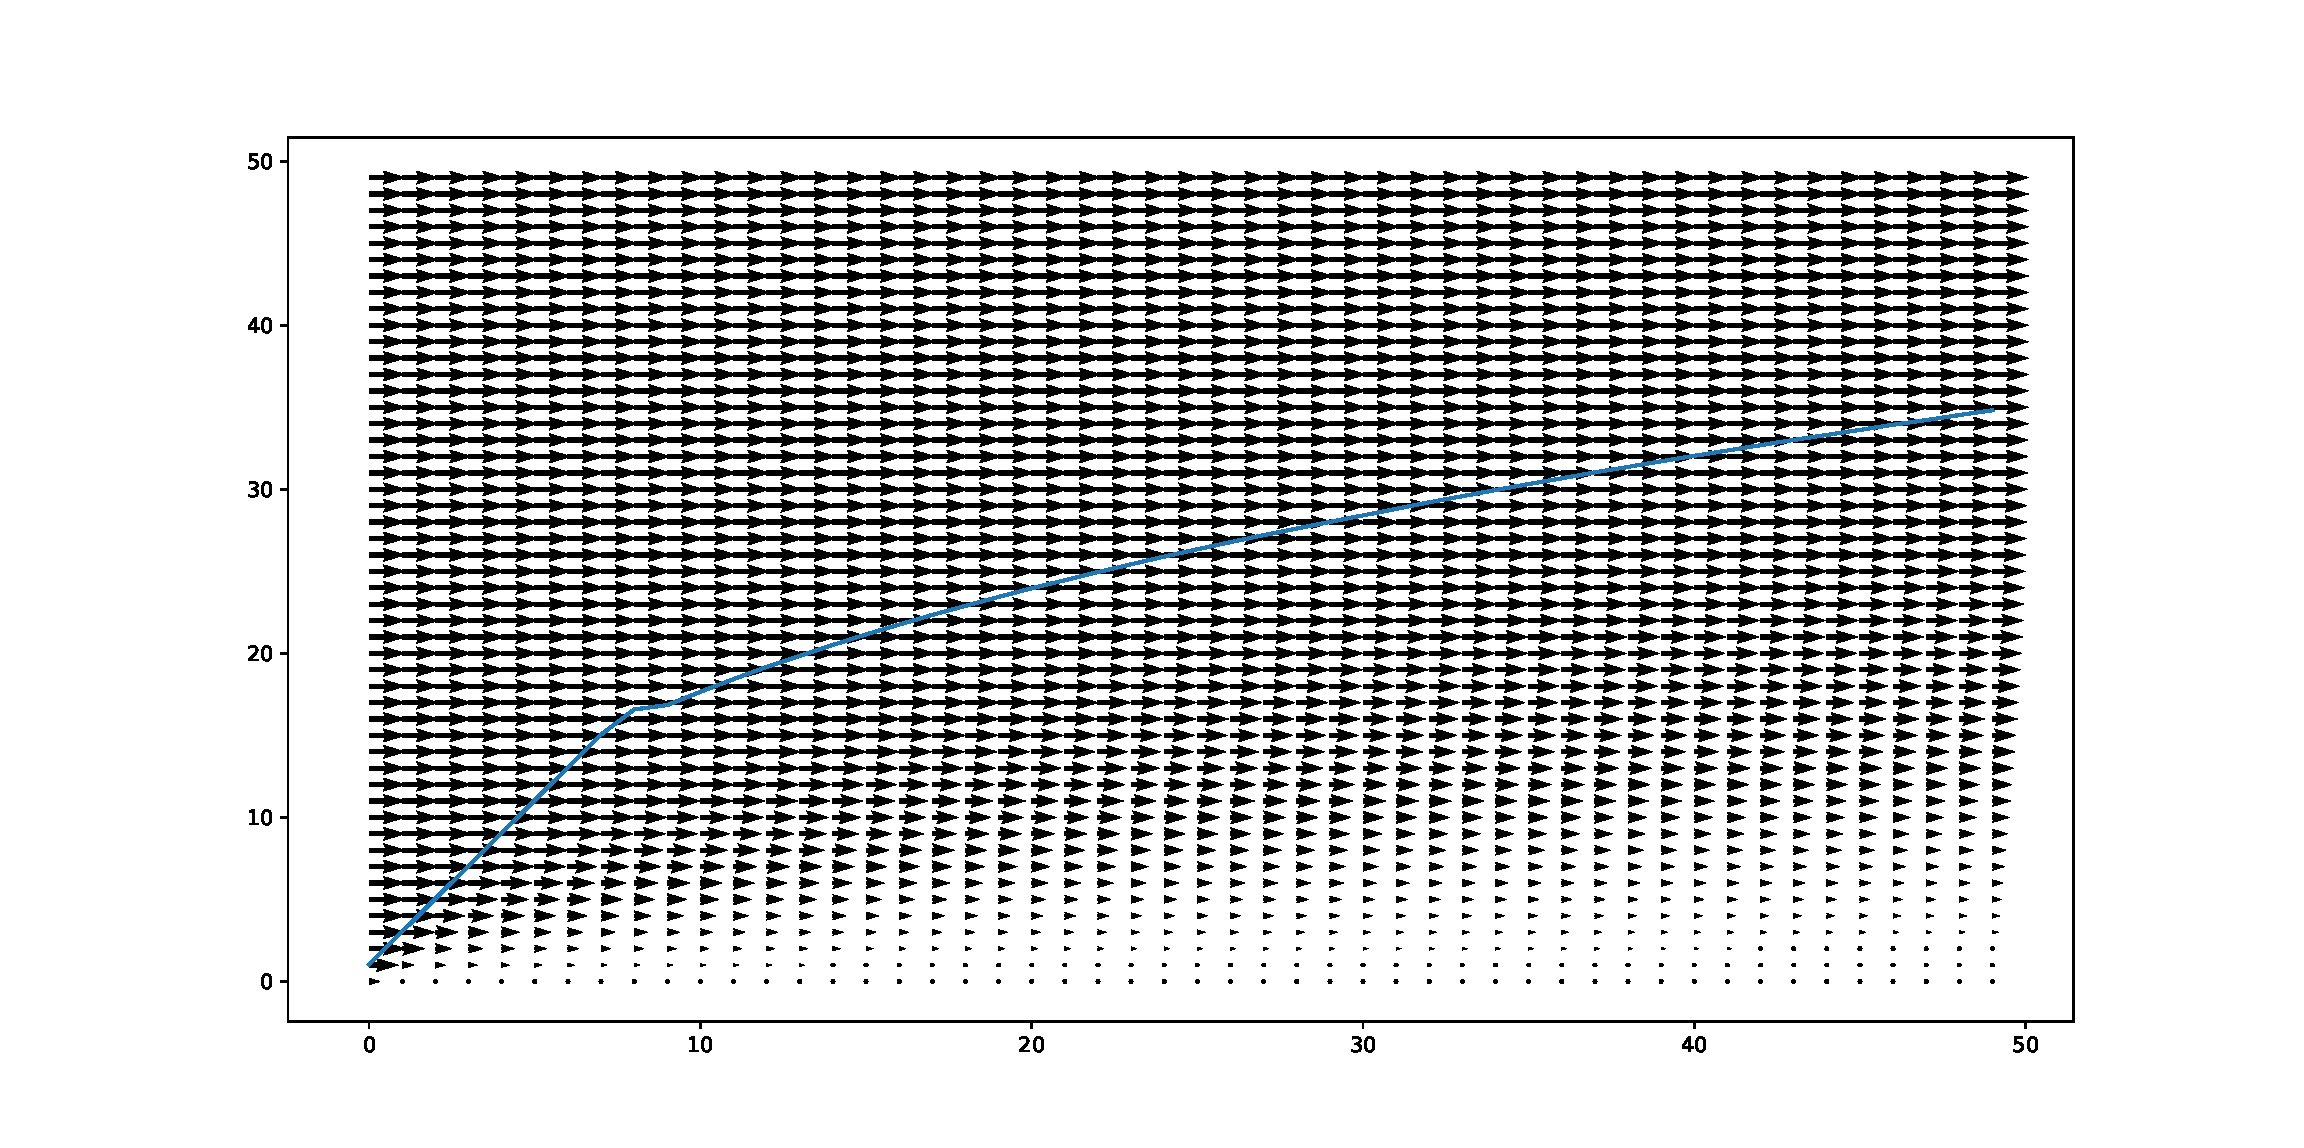
\includegraphics[width=\textwidth]{figure/dufort_stable.pdf}
        \subcaption{DuFort-Frankel法}
    \end{subfigure}
    \caption{数值解的速度场和边界层厚度,橙色线为精确解}
\end{figure}
从该图中不难看出,全显式法的解很快发散,难以求出可用的解,而DuFort-Frankel法仍能给出不错的结果,尽管解出现了比较严重的变形。

\clearpage
\appendix
\section{代码}

\subsection{全显式法}
\lstinputlisting[language=python]{code/full_explicit_solver.py}

\subsection{Du Fort-Frankel法}
\lstinputlisting[language=python]{code/dufort_frankel_solver.py}

\clearpage
\printbibliography

\end{document}
